\chapter{Experiments}
In this chapter, we evaluate the performance of the proposed approaches for skeleton-based action recognition using self-supervised learning. We start by describing the datasets used in our experiments, followed by the data preparation and processing steps. We then provide implementation details, including the architecture configurations and hyperparameters. Finally, we outline the experimental settings used for evaluation.

\section{Datasets}
For our experiments, we will evaluate our methods on two different datasets we primarily use the NTU RGB+D dataset \cite{Liu_2020}, a large-scale benchmark for 3D human action recognition for the purpose of achieving the first research objective which is developing and evaluating a contrastive self-supervised approach for action recognition on 3D human skeleton data. Then we will investigate and evaluate the proposed methods on the Drive\&Act dataset \cite{drive_and_act_2019_iccv} dedicated for driver behavior inside the car.

\begin{figure}
	\centering
	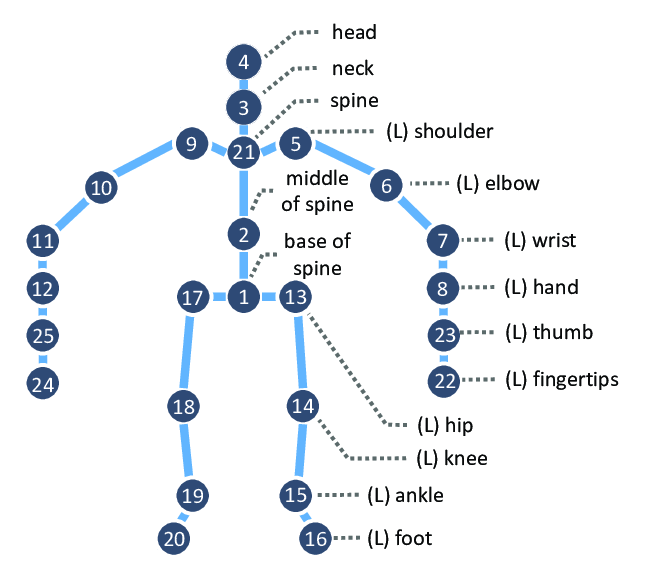
\includegraphics[width=.4\linewidth]{img/ntu_25joints.png}
	\caption{Illustration in \cite{9507447} showing the 25 joints of the human body based on NTU RGB+D.}\label{fig:ntu_25joints}
\end{figure}

\subsection{NTU RGB+D Dataset}
NTU RGB+D dataset proposed in 2016, was captured simultaneously using three Microsoft Kinect V2 sensors. It comprises 56,000 action sequences in 60 action classes, including 40 daily actions, 9 health-related actions, and 11 mutual actions. The data was collected from 40 volunteers, and each action sequence contains the three-dimensional positions of 25 body joints per frame, as shown in ~\ref{fig:ntu_25joints}. The dataset is divided into training and test sets using two different standards: Cross-Subject (X-Sub) and Cross-View (X-View). In the Cross-Subject setting, the dataset which contains 40320 samples and 16560 samples for training and evaluation, is split based on the person ID, resulting in 20 subsets for both the training and test sets. On the other hand, the Cross-View setting containing 37920 and 18960 samples for training and evaluation, divides the dataset according to camera ID. The samples collected by cameras 2 and 3 are used for training, while those collected by camera 1 are used for testing. Notably, the three cameras have horizontal angles differing by 45° each, ensuring diverse perspectives for robust evaluation.

\begin{figure}
	\centering
	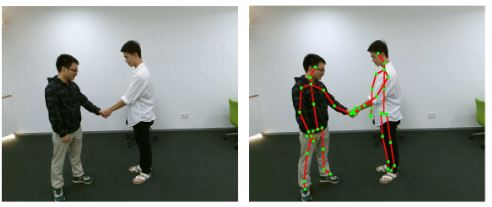
\includegraphics[width=.5\linewidth]{img/ntu_dataset.JPG}
	\caption{NTU RGB+D dataset \cite{Liu_2020} illustration of skeleton data.}\label{fig:ntu_dataset}
\end{figure}

\subsection{Drive\&Act Dataset}
The second dataset is the Drive\&Act dataset which is a significant benchmark for driver activity recognition, capturing activities in both manual and autonomous driving modes. This dataset offers a comprehensive collection of driver actions and interactions inside the vehicle cabin, providing valuable insights for driver monitoring and autonomous driving systems. The dataset consists of over 9.6 million frames, recorded from six different camera views and three modalities, collected by five Near-Infrared (NIR) and three RGB-D cameras. The data was recorded using a specially equipped vehicle that was driven on public roads in Germany. The vehicle was outfitted with six synchronized cameras placed in various positions. Three NIR cameras were utilized to capture images in low-light conditions, while three RGB-D cameras were used to capture color images and depth information. The synchronization ensured that all data streams were aligned in time, providing coherent multi-modal information for each frame. It includes skeleton data as one of its modalities. Specifically, the dataset includes 3D body and head pose data, which is represented as a time series of 3D rotation matrices. The skeleton data is captured using the OpenPose neural architecture, which is applied to each frame of the dataset that contains the driver's body or head.

The dataset comprises a hierarchical annotation scheme, offering rich semantic information about the driver's behavior. The annotations are organized into three levels:
\begin{itemize}
	\item \textbf{Coarse Tasks:} These represent high-level activities the drivers perform, such as "driving straight" or "turning left." These coarse tasks provide a broader context for understanding the driver's overall behavior.

	\item \textbf{Fine-Grained Activities:} These include more specific actions inside the vehicle cabin, such as "adjusting the radio" or "checking the rearview mirror." Fine-grained activities offer detailed insights into the driver's interactions and behaviors.

        \item \textbf{Atomic Action Units:} This level provides detailed triplets of annotations, including the driver's current action, the object they interact with, and the location of the object. This level of granularity allows for a deep analysis of the driver's actions and intentions.

\end{itemize}

The Drive\&Act dataset includes an extensive set of 83 fine-grained activity classes, surpassing previous driver activity recognition datasets by 62 additional activities. This broad range of actions enables a more comprehensive understanding of driver behavior. The dataset's size, with over 9.6 million frames, provides ample data for training and evaluation, making it one of the largest and most diverse datasets for driver activity recognition.

\begin{figure}
	\centering
	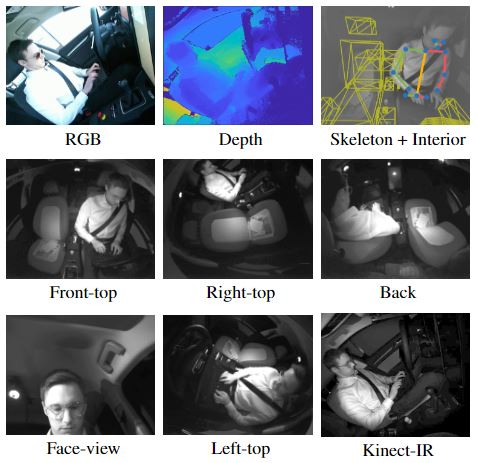
\includegraphics[width=.5\linewidth]{img/daa_dataset.JPG}
	\caption{Examples from Drive\&Act dataset \cite{drive_and_act_2019_iccv}, the "working on laptop" activity for different views and modalities.}\label{fig:ntu_dataset}
\end{figure}


\section{Data Preparation and Processing}
Preprocessing 3D skeleton data is a crucial step, considering its distinct nature compared to 2D images. In our experiments with both the NTU RGB+D and Drive\&Act datasets, we performed an in-depth analysis to gain a deeper understanding of the data and make informed decisions during preprocessing. Before diving into the preprocessing, a comprehensive visualization and analysis of the 3D skeleton data were performed. To gain a better understanding of the data, the 3D coordinates were projected onto 2 axes, allowing us to visualize the skeleton's movements and patterns, as shown in ~\ref{fig:ntu_visualisation}. This visualization helped in identifying any potential noise or inconsistencies in the data.

To improve model convergence and stability, data normalization was applied to both datasets. Normalization ensures that all 3D joint coordinates are within a consistent range, which is essential for the model's learning process. Specifically, each coordinate value was scaled to be between 0 and 1 by dividing it by the maximum value in the corresponding dimension across the entire dataset.

\begin{figure}
	\centering
	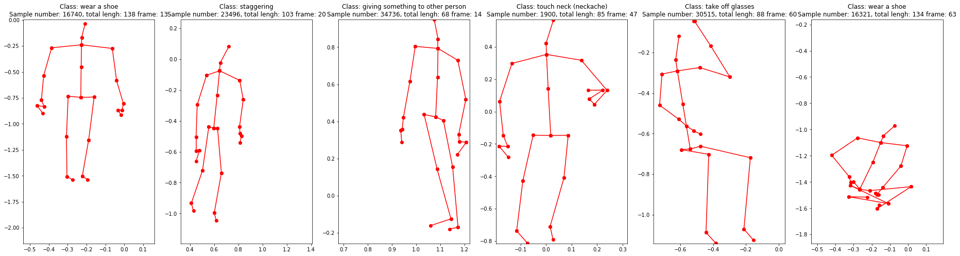
\includegraphics[width=\linewidth]{img/ntu_visualisation.png}
	\caption{Visualisations of the skeleton data from NTU RGB+D dataset plotted on x and y axes, showing the total frame of the sequence, the plotted frame, and the class label.}\label{fig:ntu_visualisation}
\end{figure}


Data augmentation is a fundamental aspect of contrastive learning, and it plays a crucial role in generating diverse views of the input skeleton sequences to enhance the model's ability to learn meaningful representations. In our preprocessing pipeline, we applied various spatial and temporal augmentations, including:

\begin{itemize}
	\item \textbf{Rotation:} An efficient spatial augmentation that randomly selected an axis (X, Y, or Z) as the main axis and applied a random rotation angle in the range [0, $\pi$/6] to it. The other two axes were also rotated with random angles in the range [0, $\pi$/180].
	\item \textbf{Crop:} As a temporal augmentation, Crop involved padding part of the frames in the original sequence and then randomly cropping it back to the original length. The padding ratio $\gamma$ was set to 1/6.
        \item \textbf{Spatial Flip:} Another spatial augmentation that swapped the left and right sides of the skeleton data with a probability of p=0.5, introducing additional variations in the data.
        \item \textbf{Shear:} A linear transformation was applied to the 3D coordinates using a shear matrix. The shear factors were randomly sampled from the range [-$\beta$, $\beta$], with $\beta$ set to 1 to control the augmentation strength.
 
\end{itemize}


\begin{figure}[htbp]
    \centering
    \subfigure{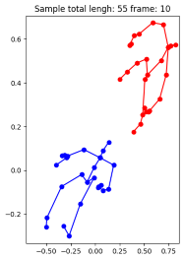
\includegraphics[width=0.3\textwidth]{img/ntu_rotation.png}}\hfill
    \subfigure{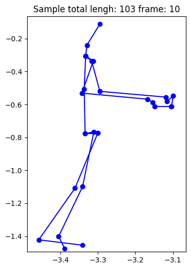
\includegraphics[width=0.3\textwidth]{img/ntu_visualisation1.png}}\hfill
    \subfigure{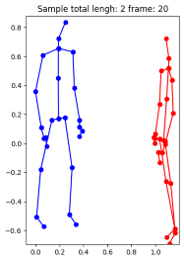
\includegraphics[width=0.3\textwidth]{img/ntu_visualisation2.png}}
    \caption{(a) Example of the rotation augmentation applied to the data. (b) Example shows a skeleton plot on the x and z axes. (c) Example shows samples with different subjects in the same frame.}
\end{figure}

These augmentations were applied to create different views of the skeleton sequences, enabling the model to capture diverse perspectives of the actions, leading to more robust and generalized representations. In addition to the ordinary augmentations described earlier, the second approach, PSTL, utilized specific masking strategies mentioned before in the Methodology chapter such as "Central Spatial Masking (CSM)" and "Motion Attention Temporal Masking (MATM)."

The data preprocessing and augmentation pipeline played a crucial role in preparing the NTU RGB+D and Drive\&Act datasets for training with the DINO and PSTL frameworks, respectively. Through visualization and analysis, normalization, and various data augmentations, we enhanced the datasets' quality and diversity, facilitating the models' ability to learn meaningful representations for effective human action recognition


The Drive\&Act dataset presented several challenges, especially when dealing with the skeleton modality. Unlike other modalities, such as RGB or NIR, only a few researchers have explored the skeleton data, making it an under-researched area. The skeleton data was extracted automatically from the N-IR modality using the OpenPose model for pose estimation. However, this led to a considerable number of errors in the annotation, including missing joints, shaded joints, and incorrect joint coordinates. Additionally, not all joints were consistently visible in the camera frame, particularly in the lower body region. Moreover, the actions in the Drive\&Act dataset exhibited similarity in terms of joint movements, making it challenging for the model to discriminate between action classes effectively. Furthermore, the dataset suffered from a significant class imbalance, with the class "sitting" being the most dominant among the 34 classes, as shown in ~\ref{fig:daa_dataset_class_visualization}.

\begin{figure}
	\centering
	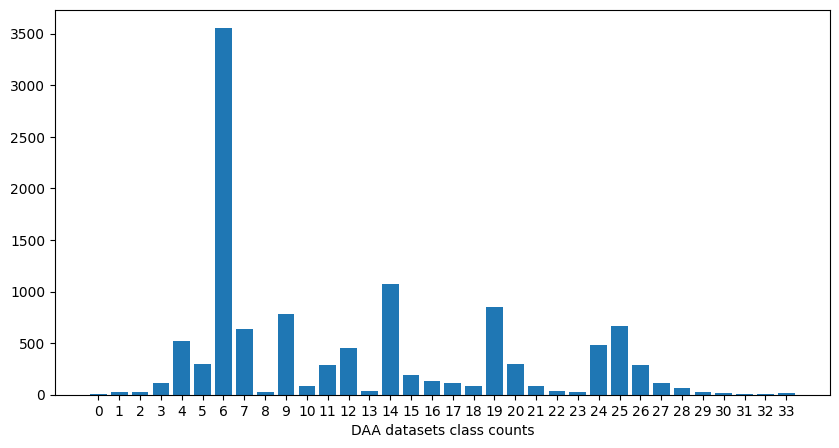
\includegraphics[width=.5\linewidth]{img/daa_dataset_class_visualization.png}
	\caption{Bar plot describing the class distribution of the Drive\&Act dataset.}\label{fig:daa_dataset_class_visualization}
\end{figure}

To address some of these issues, we decided to reduce the number of joints used in the model from 25 to 11, retaining only the most meaningful joints for better representation learning, as shown in ~\ref{fig:daa_visualization}. This will help the model focus on essential information and avoid redundancy in the data. Additionally, we employed the balanced accuracy metric during the evaluation phase to mitigate the impact of class imbalance, ensuring a fair assessment of the model's performance.

Despite the challenges and issues, the Drive\&Act dataset remains a valuable and challenging resource for driver activity recognition. Our comprehensive analysis and data preprocessing efforts aimed to create a meaningful and robust skeleton dataset, contributing to the exploration of self-supervised learning on this unique dataset. The findings from our experiments will shed light on the potential of using self-supervised learning for driver activity recognition and pave the way for future research in the Drive\&Act dataset.

\begin{figure}
	\centering
	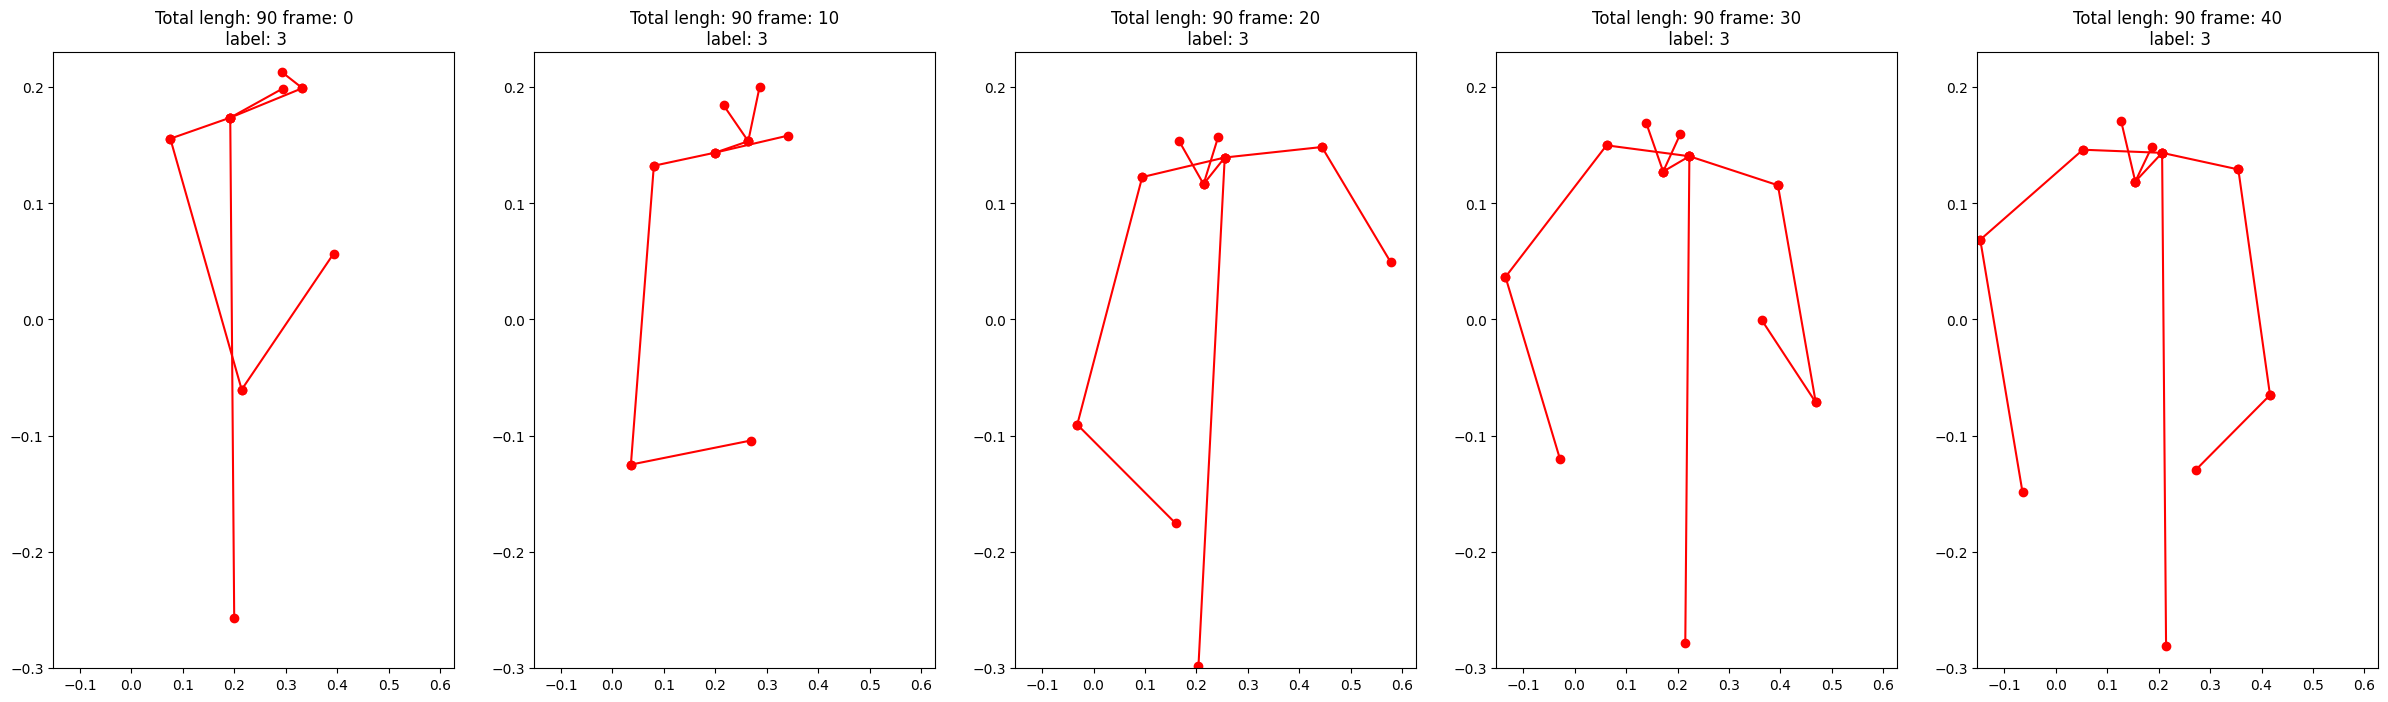
\includegraphics[width=.9\linewidth]{img/daa_sequence_visualization.png}
	\caption{Visualization of a skeleton sequence data from the Drive\&Act dataset with 11 joints. We can clearly see missing values in different frames.}\label{fig:daa_visualization}
\end{figure}

\section{Experiment Settings}
In our experimental settings, all experiments were conducted on a system equipped with 4 RTX A6000 GPUs. For the first approach, we used the NTU RGB+D dataset and the Drive\&Act dataset. To prepare the data for training, we padded the skeleton sequences to 120 frames for NTU RGB+D and 90 frames for Drive\&Act dataset. We employed the Stochastic Gradient Descent (SGD) optimizer with Nesterov momentum set to 0.9 and weight decay set to 0.0005. The loss function used was the cross entropy.

The training process for the first approach was performed over 90 epochs, with an initial learning rate of 0.3. To achieve better convergence, we used the CosineAnnealing scheduler for learning rate decay. The mini-batch size was set to 128 to balance computational efficiency and model performance. For the encoder architecture, we utilized STTFormer. In this approach, each tuple contained 6 consecutive frames, denoted as n=6. The STTFormer encoder comprised 8 spatio-temporal self-attention layers, with the output channels set to 64, 64, 128, 128, 256, 256, 256, and 256, respectively. The encoder network extracted 256-dimensional features from the skeleton sequences. To further refine the extracted features, two projectors were attached to the encoder network. Each projector consisted of 3 linear layers, with the first one followed by a batch normalization layer and leaky rectified linear units. The output size of the first linear layer was set to 512, while the final output dimension of the projector was 128.

A crucial aspect of the self-supervised learning approach is the temperature parameter, which determines the sharpness of the probability distribution. For the student network, we set the temperature parameter $\tau^s$ to 0.1, while for the teacher network, the temperature parameter $\tau^t$ was set to 0.03. This temperature scaling helped in fine-tuning the model's confidence during the contrastive learning process.

For the second approach, our experimental settings were tailored to the ST-GCN backbone and the specific requirements of PSTL. We resized the skeleton sequences to 50 frames for the NTU RGB+D dataset and 90 frames for the Drive\&Act dataset to create a suitable input length for the ST-GCN architecture.The ST-GCN backbone was configured with 16 hidden channels, which enabled the extraction of 256-dimensional features from the skeleton sequences. These features were further projected to 6144-dimensional embeddings to enhance the representation power of the model.

In the loss function of each stream, we set the value of $\lambda$ to 2e-4, which played a critical role in balancing the different components of the loss and guiding the learning process.To stabilize the training process, we utilized a 10-epoch warm-up phase, and the weight decay was set to 1e-5 to control overfitting and enhance the generalization ability of the model. During the pre-training and downstream tasks, we employed the Adam optimizer and the CosineAnnealing scheduler with 150 epochs. The mini-batch size was set to 128 for efficient computation.

For the evaluation of self-supervised learning, we utilized two protocols: linear evaluation and k-NN evaluation. In the linear evaluation, we added a linear classifier on top of the frozen pre-trained encoder and then trained the recognizer on the target skeleton action recognition dataset with an initial learning rate of 0.01. In the k-NN evaluation, we assessed the quality of features using a simple weighted k-Nearest Neighbor classifier. The pretrained model was frozen to compute and store the features of the training data for the downstream task. To classify a test skeleton $x$, we computed its representation and compared it against all stored training features, where k was set to 1. This evaluation protocol eliminated the need for hyperparameter tuning and data augmentation and could be run with only one pass over the downstream dataset, making it efficient and effective in evaluating the model's performance.

